%!TEX root = ../dokumentation.tex
\lstset{
	frame=single,
	keywordstyle=\color{blue},
	commentstyle=\color{green},
	numbers=left,
}

\chapter{Backend}

Im Backend des \textbf{Sudoku Solver} findet die Datenverarbeitung statt. Das Backend stellt das Gegenstück zum Frontend dar. In diesem Kapitel wird die Programmarchitektur beschrieben und die wichtigsten Klassen des Backend vorgestellt. Hier werden auch alle umgesetzten Lösungstechniken aufgezählt und bereits einen kleinen Ausblick gegeben welche Strategien noch weiter implementiert werden könnten. Danach wird die Umsetzung der Strategien beispielhaft an zwei Strategien erklärt.

\todo{Übergang schreiben, was alles im Backend}

\section{Programmarchitektur}
\todo{UML}


\section{Serverseite}

\todo{Serverseite}

In den meisten Fällen wird die Verbindung über WebSocket hergestellt, was einen Kommunikationskanal mit geringem Aufwand zwischen Server und Client darstellt. Für die Studienarbeit wird für die Kommunikation SocketIO verwendet. 

\subsection{SocketIO}

Socket.IO ist eine Bibliothek, die eine bidirektionale und ereignisbasierte Kommunikation mit niedriger Latenz zwischen einem Client und einem Server ermöglicht. Die Hauptidee hinter Socket.IO ist, dass beliebige Ereignisse mit beliebigen Daten gesendet und empfangen werden können.

Auf der Server-Seite erweitert die Socket-Instanz die EventEmitter-Klasse.

Auf der Client-Seite verwendet die Socket-Instanz den Ereignis-Emitter, der von der Komponenten-Emitter-Bibliothek bereitgestellt wird, die eine Teilmenge der EventEmitter-Methoden bereitstellt.

\section{SudokuBoard}

Ein wichtiger Part des Backend ist die Klasse des \textit{SudokuBoard}. In dieser Klasse wird das Sudokuboard erstellt und eine Datenstruktur erschaffen in der die Informationen gespeichert werden. Aufgrund dieser Datenstruktur werden die Lösungsstrategien angewendet. In diesem Abschnitt wird die Datenstruktur erläutert und einige Funktionalitäten des SudokuBoard vorgestellt.

Die Zahlen und Kandidaten werden in unterschiedlichen Listen gespeichert. Das Board besteht aus einer zweidimensionalen List und die Kandidatennotation wurde mithilfe einer dreidimensionalen Liste umgesetzt. Für das Projekt wurde die Datenstruktur von Zambon \cite{zambon2015sudoku} repliziert. 

\subsection{Datenstruktur des Sudokuboards}
Die Zellenidentifikation ist in Abbildung \ref{fig:Sudokugitter} dargestellt. Der Inhalt der Zellen wird in einer Zweidimensionalen Liste gespeichert. Mit dem ersten Index wird eine Spalte ausgewählt und mit dem zweiten Index die Spalte. 

\begin{figure}[htbp]
	\centering
	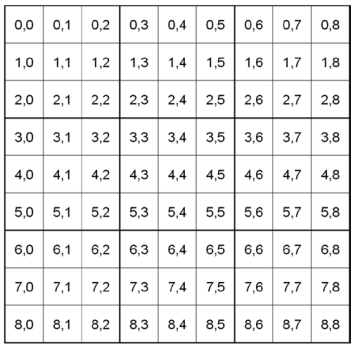
\includegraphics[width=0.3\textwidth]{images/board.png}
	\caption{Struktur des Sudokuboards und Zellenidentifikation \cite{zambon2015sudoku}}
	\label{fig:Sudokugitter}
\end{figure}

Wenn noch kein Board initialisiert wurde, dann wird die Datenstruktur erstellt und das gesamte Board mit Nullen befüllt. Diese Funktion ist in dem Codebeispiel \ref{lst:board} 

\begin{lstlisting}[caption={Initalisierung des Boards}, label={lst:board}]
	def init_board(self):
		self.board = []
		for i in range(SIZE):
			self.board.append([])
			for j in range(SIZE):
				self.board[i].append(0)
\end{lstlisting}

Die Kandidaten sind in einer dreidimensionalen Liste gespeichert. Mit den ersten beiden Indizes werden, genau wie auf dem Board die Zellen identifiziert. Der dritte Index gibt Informationen über die Kandidaten die in einer Zelle stehen. Die Kandidaten werden über Flags gesetzt. Das bedeutet, dass man in der innersten Liste überprüfen muss an welcher Stelle eine eins steht. Indizes an denen eine eins steht müssen um eins inkrementiert, um den konkreten Kandidatenwert zu ermitteln, denn die Listen starten immer mit dem Index Null. 

\begin{lstlisting}[caption={Initalisierung der Kandidaten}, label={lst:candiates}]
	def init_candidates(self):
		for i in range(SIZE):
			self.candidates.append([])
			for j in range(SIZE):
				self.candidates[i].append([1] * SIZE)
\end{lstlisting}

Beim initialisieren der Kandidaten, wie im Code \ref{lst:candidates} umgesetzt, werden zunächst alle Kandidaten gesetzt. Auf einem leeren Board könnte nämlich in jede Zelle jeder Wert, wenn noch keine Zahlen vorgegeben sind. Sobald dann Zahlen eingetragen werden, werden die Kandidatenwerte geupdated.

\subsection{Funktionalität}
Neben der Initialisierung des Boards und der Kandidaten, gehört das Prüfen der eindeutigen Lösbarkeit eines Sudokurätsel zu den wichtigsten Funktionalitäten der \textit{SudokuBoard} Klasse. Diese Umsetzung dieser Funktionen wurde in dem Abschnitt \ref{eindeutigLösbar} und dem nächsten bereits vorgestellt. Eine weiter wichtige Funktionalität dieser Klasse ist das updaten des Boards und der Kandidaten wenn Zahlen eingetragen sind. Auf diesen Datenstrukturen bauen alle Umsetzungen der Lösungstechniken auf. 

Des weiteren findet im \textit{SudokuBoard} die Umsetzung der Strategien statt. Dafür wurden die FUnktionen \textit{remove\_candidates(self, cross\_outs)} und \textit{update\_numbers(self, number, cells)} implementiert. 




\section{Technique Manager}
In der Datei \textit{technique\_manager.py} wird das Aufrufen der Techniken geregelt. Alle Lösungsstrategien sind als Klassenrepräsentation der umgesetzten Technik in einer Liste gespeichert. Über diese Liste wird drüber iteriert und das Board und die Kandidaten übergeben. Danach wird die abstrakte Methode \textit{execute\_technique()} für die Lösungstechnik ausgeführt. Der Returnwert dieser Methode ist True, wenn sich etwas an dem Board oder an den Kandidaten verändert. In diesem Fall wird die Methode \textit{get\_result()} aufgerufen, mit der die Änderungen durchgeführt werden können.
Wenn eine Technik nicht erfolgreich ist dann wird mit der nächsten Lösungsstrategie aus der Liste weiter gemacht. 

Die Reihenfolge der Lösungstechniken ist von der Website \cite{martin} übernommen. Zuerst werden einfache Lösungsansätze ausprobiert und wenn diese nicht erfolgreich sind, werden immer komplexere Techniken angewendet. 

\begin{lstlisting}[language=Python, caption={Funktion um eine anwendbare Lösungstechnik zu finden}, label={lst:try}]
	def try_techniques(board, candidates):
		for tech in techniques:
			technique = tech(board, candidates)
			successful = technique.execute_technique()
			if successful:
				return technique.get_result()
		return False
\end{lstlisting}

\section{Abstrakte Klasse SolvingTechniques}

Wie im vorherigen Abschnitt des Technique Manager schon erwähnt gibt es eine Abstrakte Klasse Namens \textit{SolvingTechniques}, deren Funktionsweiße und Vorteile im weiteren Verlauf des Absatzes erläutert wird. 

Mit einer Abstrakten Klasse kann ein gemeinsames Verhalten definiert werden. Dieses Verhalten wird von mehreren Unterklassen geerbt. Der Unterschied zwischen Klassen und abstrakten Klassen ist, dass von abstrakten Klassen weder Objekte erstellt werden können, noch dass sie instanziiert werden können. Der Vorteil einer abstrakten Basisklasse ist die Nutzung mehrerer Unterklassen an einer gemeinsamen Programmierschnittstelle, in diesem Fall in dem \textit{TechniqueManager}. Zudem wird das gesamte Projekt durch das Einführen einer abstrakten Klasse übersichtlicher, dar alle Unterklassen von dieser einen Klasse erben.

Diese abstrakte Klasse macht es dem Technique Manager möglich, alle Klassen der Lösungstechniken auf die selbe Weise zu instanziieren und zu verwenden. Mithilfe der abstrakten Klasse wird die Struktur der Lösungstechniken verallgemeinert, ohne dass jede Methode vollständig implementiert ist. 

Neben abstrakten Methoden sind noch weitere Funktionen in dieser Klasse implementiert die in mehreren Unterklassen verwendet werden können. Wenn eine Klasse also von einer abstrakten Klasse abgeleitet ist, so müssen alle abstrakten Methoden implementiert und überschrieben werden. 

\subsection{Abstrakte Methoden}
Die Verallgemeinerung der Lösungstechniken wird über abstrakte Methoden umgesetzt. Diese Methoden bieten die Standardfunktionalitäten der Basisklassen und müssen, wie schon erwähnt, implementiert werden. In Python können abstrakte Klassen erstellt werden, indem sie von dem ABC-Modul erben.

In der abstrakten Klasse \textit{SolvingTechniques} sind unter anderem drei verschiedene abstrakte Methoden deklariert. Diese brauchen in der abstrakten Klasse selbst keine Implementierung. Jede Klasse der Lösungstechniken braucht die Funktionen \textit{execute\_technique(self)}, \textit{configure\_highlighting(self)} und \textit{update\_explanation(self)}.

Mithilfe dieser drei abstrakten Methoden können alle Lösungstechniken übersichtlich implementiert werden. Nach Ausführen dieser Methoden wurde die Lösungstechnik auf das Sudoku angewendet. Dabei  wurden verschiedene Informationen in Variablen hinterlegt, die für den User mit der weiteren Benutzung der Hilfestellungen relevant sind.
Die Funktion der einzelnen Methoden wird in den folgenden Abschnitten erläutert. Im Zuge dessen werden auch die für das Frontend bereits erwähnten und wichtigen Variablen vorstellt, sowie der Grund des Erstellens.

\subsubsection{execute\_technique(self)}
In der Methode \textit{execute\_technique(self)} werden die Algorithmen für die spezifischen Techniken implementiert. Dabei wird zunächst nur überprüft, inwiefern eine Technik anwendbar ist. 

Wenn ein Algorithmus ein Muster für eine Technik erkennt und in der nächsten Methode Kandidaten zum raus streichen gefunden werden, wird der Wert True zurückgegeben. Wenn keine passende Konstellation gefunden wird oder die Technik keine Auswirkung auf das aktuelle Board hat, dann wird ein False zurückgegeben.

\subsubsection{configure\_highlighting(self)}
Wenn ein Algorithmus eine Technik gefunden hat, dann wird in \textit{execute\_technique(self)} die abstrakte Methode 
\textit{configure\_highlighting(self)} aufgerufen. 

In dieser Methode werden die spezifischen Zellen und Kandidaten in denen die Technik gefunden wurde markiert. Dafür wurden in \textit{SolvingTechniques} Klassenvariablen angelegt. 
\begin{itemize}
	\item \textit{self.cross\_outs = []}
	\item \textit{self.highlights = []}
	\item \textit{self.primary\_cells = []}
	\item \textit{self.secondary\_cells = []}
\end{itemize}

Diese Variablen haben wir schon im Frontend im Abschnitt \ref{Abstufung} kennengelernt und deren Bedeutungen beschrieben. In den \textit{self.cross\_outs} werden Kandidaten in bestimmten Zellen gespeichert, die laut Strategie entfernt werden können und in den \textit{self.highlights} werden Kandidaten aus bestimmten Zellen gespeichert, die eine besondere Bedeutung für die Strategie haben. Die \textit{self.primary\_cells} und \textit{self.secondary\_cells} enthalten nur Zellen, die für die Strategie relevant sind. Dabei sind die \textit{self.primary\_cells} tendenziell relevanter für Strategien und werden deutlicher hervorgehoben im Gegensatz zu den \textit{self.secondary\_cells}.

\subsubsection{update\_explanation(self)}
In \textit{update\_explanation(self)} wird eine Erklärung der Strategie gegeben. Diese Erläuterung wird in der Klassenvariable \textit{self.explanation} gespeichert. Bei der Erklärung wird darauf geachtet die Strategie an dem gefundenen Beispiel zu erläutern und den Grund zu nennen warum man diese Technik anwenden kann.

\subsection{Hilfsfunktionen}

In der abstrakten Klasse gibt es zusätzlich zu den abstrakten Methoden noch weitere Hilfsfunktionen. Diese Funktionen können in den Unterklassen aufgerufen werden, um die Implementierung zu erleichtern. Zu den wichtigsten Hilfsmethoden gehört \textit{get\_influential\_cells\_unit(cell, unit)}. Diese Methode gibt zu einer Zelle und einer Unit, alle Zellen die von der übergebenen Zelle in der spezifischen Unit gesehen werden, zurück. Für viele Strategien dient diese Funktion als Ausgangspunkt um bestimmte Muster auf dem Board zu erkennen.

Eine weitere sehr wichtige Methode ist \textit{get\_result(self)}. In dieser Methode werden die in \textit{configure\_highlighting(self)} gesammelten Informationen, der Technikname und die in der der Methode \textit{configure\_highlighting(self)} angepasste Beschreibung returnt. Die Informationen werden in einem Dictionary gespeichert und übergeben. Damit man auf alle nötigen Variablen zurückgreifen kann, wurde diese Variablen als Klassenvariablen angelegt. Die in den Unterklassen gespeicherten Informationen können in der abstrakten Klasse verwendet werden.

\section{Lösungsstrategien}

In diesem Abschnitt wird ein Überblick über die implementierten Strategien gegeben. Die Lösungsstrategien sind auf der Website von Simon Martin \cite{martin} betitelt und beschrieben. Anhand diesen Beschreibungen wurden einige Lösungsstrategien implementiert. Zunächst wird ein Überblick über die umgesetzten Strategien gegeben, bevor ausblickend die Lösungsstrategien, die noch nicht implementiert wurden, aufgezählt werden. Es gibt noch weitere Strategien die auf der Website nicht beschrieben werden. Diese werden im Folgenden aber nicht weiter beachtet.

\subsection{Umgesetzte Lösungsstrategien}
Da in der Ausarbeitung nur exemplarisch auf einige wenige Lösungsstrategien eingegangen wird, sind in der Tabelle \ref{tab:implStrategien} alle implementierten Lösungsstrategien aufgezählt.
% Please add the following required packages to your document preamble:
% \usepackage{graphicx}
\begin{table}[H]
	\centering
	\resizebox{\textwidth}{!}{%
		\begin{tabular}{lllll}
			\cline{1-2} \cline{4-5}
			Technikname               & Technikname engl.          &  & Technikname               & Technikname engl.          \\ \cline{1-2} \cline{4-5} 
			Versteckter Single        & HiddenSingle               &  & Nackter Single            & Naked Single               \\
			Verstecktes Paar          & Hidden Pair                &  & Nacktes Paar              & Naked Pair                 \\
			Versteckter Dreier        & Hidden Triple              &  & Nackter Dreier            & Naked Triple               \\
			Versteckter Vierer        & Hidden Foursome            &  & Nackter Vierer            & Naked Foursome             \\
			Reihe-Block-Check         & Line-Block-Interaction     &  & Block-Reihe-Check         & Block-Line-Interaction     \\
			X-Wing                    & X-Wing                     &  & Steinbutt                 & Turbot                     \\
			Drittes Auge              & Third Eye                  &  & Wolkenkratzer             & Skyscraper                 \\
			Schwertfisch              & Swordfish                  &  & Drachen                   & Dragon                     \\
			Verbotenes Rechteck Typ 1 & Forbbiden Rectangle Type 1 &  & Verbotenes Rechteck Typ 2 & Forbbiden Rectangle Type 2 \\
			Verbotenes Rechteck Typ 3 & Forbidden Rectangle Type 3 &  & Verbotenes Rechteck Typ 4 & Forbidden Rectangle Type 4 \\
			XY-Wing                   & XY-Wing                    &  & XYZ-Wing                  & XYZ-Wing                   \\
			X-Kette                   &                            &  & XY-Kette                  & XY-Chain                   \\
			Schwertfisch mit Flosse   & Swordfish with fin         &  & W-Wing                    &                            \\
			Geklonte Paare            &                            &  & Leeres Rechteck           &                            \\
			Doppelkette               & Double Chain               &  & Forcing Chain             &                            \\ \cline{1-2} \cline{4-5} 
		\end{tabular}%
	}
	\caption{Aufzählung aller implementierten Lösungsstrategien mit deutschem und englischem Bezeichner}
	\label{tab:implStrategien}
\end{table}

\todo{Tabelle endgültiger Stand}

\subsection{Weitere Lösungsstrategien}
In der Studienarbeit wurden nicht alle auf der Website \cite{martin} vorgestellten Lösungstechniken umgesetzt. Weitere Strategien die noch implementiert werden könnten sind die folgenden:
\begin{itemize}
	\item Erweiterter \ac{BRC}
	\item (noch nicht) X-Kette
	\item (noch nicht) W-Wing
	\item (noch nicht) Geklonte Paare
	\item (noch nicht) Leeres Rechteck
	\item Forcing Chain
\end{itemize}

\todo{Liste aktueller Sand}

Der Erweiterte \ac{BRC} wurde nicht umgesetzt, weil es eine Kombination aus dem \ac{BRC} und einem Versteckten Single ist. Außerdem wurde die Forcing Chain nicht implementiert, weil die Technik gleich ist mit der XY-Kette.

\section{Beispielhafte Umsetzung von Strategien}
Die Lösungsstrategien können zwei unterschiedliche Wirkungen auf ein Sudokurätsel haben. Entweder es ist möglich eine Zahl einzufügen oder es können Kandidaten aus verschiedenen Gründen eliminiert werden. Diese beiden Wirkungen werden im Backend unterschiedlich behandelt. In den nächsten zwei Unterkapiteln wird die Funktionsweise und die Unterschiede beider Varianten anhand zweier Beispiele erklärt. 

Für beide Umsetzungen wird die Abstrakte Klasse \textit{SolvingTechniques} genutzt.

\subsection{Zahl einfügen}

Der Fall, dass aufgrund einer Lösungstechnik direkt eine Zahl in das Sudokugitter eingetragen werden kann, gibt es nur bei drei Techniken. Für alle anderen Techniken ist das eintragen einer Zahl maximal das Resultat von dem Herausstreichen einer Zahl. 
\begin{itemize}
	\item Versteckter Single
	\item Nackter Single
	\item Drittes Auge
\end{itemize}

Für das Beispiel wird die Strategie des Versteckten Single erklärt.

Sobald auf dem Numpad der Help Button das erste mal gedruckt wird, wird die Funktion \textit{try\_techniques()} im \textit{TechniqueManager} ausgeführt. 
\begin{lstlisting}[caption={Serverseitig help}, label={lst:helper}]
@socketio.on('help')
def help():
	global help_step
	global technique_result
	...
	if help_step == 0:
		sudoku.update_candidates()
		technique_result = technique_manager.try_techniques(sudoku.board, sudoku.candidates)
		if not technique_result:
			print("No suitable technique found!")
			return
		emit('help0', {'name': technique_result['name'], 'primaryCells': technique_result['primary_cells'], 'secondaryCells': technique_result['secondary_cells']})
\end{lstlisting}

Zunächst wird die List der Techniken im \textit{TechniqueManager} durch iteriert. An der Stelle des Versteckten Single wird von der abstrakten Methode \textit{execute\_technique(self)} True zurückgegeben. Die Funktion ist in dem Codebeispiel \ref{lst:NakedSingle} abgebildet. Der Algorithmus loopt über alle Zellen auf dem Board. Wenn in einer Zelle eine Zahl steht die nicht Null ist, dann wird diese übersprungen. Als nächstes wird überprüft ob die Summe der Kandidaten in diesem Felder ungleich eins ist. Wenn also mehrere Kandidaten in einer Zelle sind, so wird auch diese übersprungen. Wenn eine Zelle nur einen Kandidaten hat, dann wird in dieser Zelle ein Nackter Single erkannt und zu den \textit{self.primary\_cells} hinzugefügt. Als nächstes wird die abstrakte Funktion \textit{configure\_highlighting(self)} aufgerufen und dann True returnt. 

\begin{lstlisting}[caption={Nackter Single}, label={lst:NakedSingle}]
	def execute_technique(self):
		for i in range(9):
			for j in range(9):
				if self.board[i][j] != 0:
					continue
				if sum(self.candidates[i][j]) != 1:
					continue
				self.primary_cells = [(i, j)]
				self.configure_highlighting()
				return True
		return False
\end{lstlisting}

Daraufhin wird die Hilfsmethode \textit{get\_result()} für das Objekt des Versteckten Single aufgerufen. Diese Ergebnisse sind nun in der globalen Variable \textit{technique\_result} gespeichert. Wenn nichts in der Variable steht, dann hat das Programm keine passende Technik gefunden. Für jede weitere Hilfestellung wird der \textit{help\_step} um eins erhöht. Über emit kann ein Event, dessen Callback in diesem Fall 'help0' ist, ausgeführt werden. Die 'help0' Funktion wurde im Frontend in dem Abschnitt \ref{Abstufung} vorgestellt. Mit dem emit werden zudem die gebrauchten Informationen übergeben.

Die nächsten beiden Hilfestellungen funktionieren auf die selbe Art und Weise. Erst bei der letzten Hilfestellung, dem Anwenden der Strategie, wird die einzig nötige Unterscheidung getroffen. Wie in dem Codebeispiel \ref{lst:helper1} gezeigt, wir der Name der Technik abgefragt. Wenn es eine der drei Techniken ist, bei denen eine Zahl auf dem Gitter eingefügt, dann wird die Funktion \textit{new\_number()} aufgerufen. Dieser Funktion wird die Zelle und der Kandidatenwert übergeben, in die der Wert eingetragen werden muss. Diese Werte bekommt man aus den \textit{self.highlights}.

\begin{lstlisting}[caption={Serverseitige Unterscheidung der zwei Arten von Techniken}, label={lst:helper1}]
	elif help_step == 3:
		if technique_result['name'] in ['Naked Single', 'Hidden Single', 'Third Eye']:
			data = {'number': technique_result['highlights'][0]['value'], 'checkedCells': [technique_result['highlights'][0]['cell']]}
			emit('help3')
			new_numbers(data)
			help_step -= 1
		else:
			sudoku.remove_candidates(technique_result['cross_outs'])
			candidates()
			emit('help3')
\end{lstlisting}

%Da die serverseitige Implementierung hier aufgeteilt vorgestellt wird, ist die ganze Funktion nochmals im Anhang \ref{lst:helpers} zu sehen.

\subsection{Kandidaten eliminieren}

Die Funktionsweise von Strategien die Strategien eliminieren ist ähnlich wie gerade beschrieben. Der einzige Unterschied ist, dass anstatt \textit{new\_number()} die Funktion \textit{remove\_candidate()} aufgerufen wird. Der optische Output wird wieder über emits organisiert. Aus diesem Grund wird für die Lösungsstrategie Versteckter Vierer nur die \textit{execute\_technique(self)} erläutert. 

Da diese Technik in jeder Unit vorkommen könnte, wird zu Beginn über alle drei Units geloopt. Da es jede Unit neun mal gibt wird ebenso über über diese neun Units geloopt. Im folgenden Schritt werden alle Zellen einer Unit gespeichert. Über diese Zellen einer Unit wird drüber geloopt und Zellen in denen schon Zahlen stehen werden übersprungen. Wenn in einer Zelle aber nur Kandidaten gespeichert sind, dann wird der Wert der Kandidaten in der Liste \textit{occurring\_candidates} gespeichert. Auf den Wert des Kandidaten kommt man aufgrund der Datenstruktur von den Kandidaten, indem man die Stelle an der sie in der Kandiadtenliste durch eine 1 gekennzeichnet sind um eins inkrementiert. Die Umsetzung ist in dem Codebeispiel \ref{lst:hiddenFoursome1}

\begin{lstlisting}[caption={Erster Teil der Strategie Versteckter Vierer}, label={lst:hiddenFoursome1}]
	def execute_technique(self):
		for self.unit in ['row', 'column', 'box']:
			for j in range(9):
				...
				self.unit_cells = SolvingTechniques.get_influential_cells_unit((j, i), self.unit)
				for cell in self.unit_cells:
					...
					for num, candidate in enumerate(self.candidates[x][y]):
						if candidate == 0:
							continue
						if num + 1 not in occurring_candidates:
							occurring_candidates.append(num + 1)
\end{lstlisting}


Als nächstes wird aus der Liste der Kandidaten die in einer Unit gefunden wurden, alle möglichen Kombinationen gebildet in denen diese Kandidaten in einer Zelle vorkommen könnten. Für alle Kombinationen wird erneut über die Zellen der Unit iteriert. In den Zellen wird mittels einer Listcomprehension überprüft ob ausschließlich Kandidaten aus der Kombination vorkommen. Wenn die Überprüfung erfolgreich ist wird die Zelle zur Liste \textit{matches} hinzugefügt. Nachdem über alle Zellen iteriert wurde, wird die lange der Liste an Übereinstimmungen überprüft. Für den Versteckten Vierer müssen vier Zellen in der List vorkommen. Dieser Teil der Strategie ist in dem Codebeispiel \ref{lst:hiddenFoursome2} implementiert.

Der vorletzte Schritt ist das Festlegen der Markierungen. Dafür wird hier wie zuvor beschrieben die abstrakte Methode \textit{configure\_highlighting(self)} aufgerufen. Als letztes wird überprüft ob Kandidaten herausgestrichen werden können. Wenn die Liste der \textit{self.cross\_outs} größer als Null ist, dann wird der Wert True zurückgegeben. Wenn keine Kandidaten herausgestriuchen werden können, dann wird mit der nächsten Unit auf die zuvor beschriebene Art und Weise verfahren.

\begin{lstlisting}[caption={Erster Teil der Strategie Versteckter Vierer}, label={lst:hiddenFoursome2}]
	combos = set(combinations(occurring_candidates, 4))
	for self.combo in combos:
		matches = []
		for cell in self.unit_cells:
			...
			candidates_num = SolvingTechniques.format_candidates(self.candidates[x][y])
			if any(c in self.combo for c in candidates_num):
				matches.append(cell)
		if len(matches) == 4:
			self.primary_cells = matches
			self.configure_highlighting()
			if len(self.cross_outs) != 0:
				return True
\end{lstlisting}

Wenn in keiner Unit ein versteckter Vierer entdeckt wird von dem Algorithmus, dann gibt die Funktion False zurück und das Programm macht mit der nächsten Lösungsmethode weiter.